\section{Binary Junction Transistors}\label{sec:BJTs}
\begin{definition}[BJT]\label{def:BJT}
  The \emph{BJT}, short for \emph{Binary Junction Transistor}, is another important \nameref{def:Transistor}.

  The physical structure of both \NPNTransistor{}s and \PNPTransistor{}s is shown in \Cref{fig:BJT-NPN-Physical_Structure,fig:BJT-PNP-Physical_Structure}.

  \begin{remark}[Emitter-Collector Notation]
    The emitter of the \nameref{def:BJT} is named so because of the way we define current.
    We actually define current to be the reverse flow of electrons (not technically the holes).
    Thus, the emitter emits ``negative electrons''.

    The collector collects the electrons that have been injected.
    Because we consider current to be the opposite direction of the flow of electrons in a circuit, the collector's current is denoted as moving inwards, even when the electrons are flowing outwards.
  \end{remark}
\end{definition}

\begin{figure}[h!tbp]
  \centering
  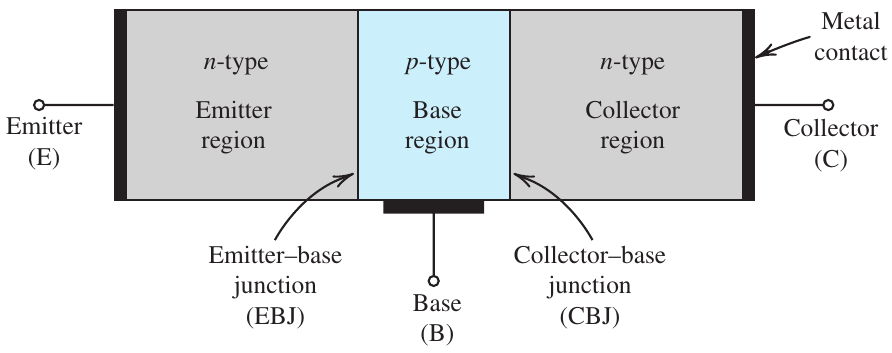
\includegraphics[scale=0.75]{./BJT-NPN-Physical_Structure.png}
  \caption{\NPNTransistor{} Physical Structure \parencite[p.~307]{sedraTextbook7}}
  \label{fig:BJT-NPN-Physical_Structure}
\end{figure}


%%% Local Variables:
%%% mode: latex
%%% TeX-master: "../ECE_311-Engineering_Electronics-Reference_Sheet"
%%% End:
